\documentclass[]{article}

\usepackage{amsmath}
\usepackage{multirow}
\usepackage{natbib}
\usepackage{graphicx} 
\usepackage{tabularx}
\usepackage{booktabs}

\begin{document}

\title{Accelerating Critic Learning via Lyapunov-Structured Value Functions for Reinforcement Learning}

\author{Denario}
\date{Anthropic, Gemini \& OpenAI servers. Planet Earth.}

\maketitle
\begin{abstract}
Learning accurate value functions from scratch is a key challenge contributing to the sample inefficiency of deep reinforcement learning in continuous control. To address this, we investigate incorporating control-theoretic priors by structuring the critic's value function as the sum of a known analytic Lyapunov function and a learned neural network residual. We evaluated this approach using the Proximal Policy Optimization (PPO) algorithm on the Gymnasium Pendulum-v1 stabilization task, comparing a standard agent against one with the Lyapunov-structured critic. Our results show that the structured critic converged substantially faster, achieving an 87\% lower overall training loss and an 8-fold reduction in loss during early training compared to the baseline. Furthermore, the resulting value function was 86\% closer to the analytic Lyapunov function. However, these significant improvements in value function approximation did not translate into superior policy performance or sample efficiency within the 100,000-step training horizon, as neither agent learned a stable policy. These findings suggest that while Lyapunov structural priors can dramatically accelerate value function convergence, the realization of corresponding policy improvements in on-policy algorithms may require a more extensive training budget.
\end{abstract}








\section{Introduction}
\label{sec:intro}
Deep reinforcement learning has emerged as a powerful paradigm for solving complex sequential decision-making problems. However, its application to continuous control tasks, particularly in robotics and physical systems, is often hampered by substantial sample inefficiency. A primary contributor to this challenge is the difficulty of learning an accurate value function, which estimates the expected long-term return from a given state and guides policy improvement. In standard implementations, the value function is approximated by a neural network trained from scratch. This \textit{tabula rasa} approach disregards available domain knowledge, forcing the agent to discover the underlying dynamics and task structure through extensive and often costly trial-and-error interaction with the environment.

In contrast, classical control theory provides a mature framework for analyzing and controlling dynamical systems, often leveraging analytical models. Lyapunov stability theory, in particular, offers a rigorous method for certifying system stability around an equilibrium point. This is achieved through a Lyapunov function: a scalar, energy-like function of the system's state that is positive definite and decreases along all system trajectories. The existence of such a function provides a formal guarantee of convergence to the equilibrium. For many physical systems, an analytical Lyapunov function can be derived from first principles, representing a potent piece of prior knowledge about the system's behavior.

The objective of a Lyapunov function—to decrease towards a minimum at a stable equilibrium—bears a strong conceptual resemblance to the optimal value function in a reinforcement learning stabilization task. This parallel suggests a promising opportunity to fuse the strengths of both domains: using a known Lyapunov function as a structural prior to guide the value function learning process. Instead of requiring a neural network to learn the entire value landscape from a random initialization, we can initialize it with a physically meaningful approximation. The learning problem is thereby reframed from discovering the full function to learning a smaller, potentially simpler residual correction that accounts for model inaccuracies or complex dynamics not captured by the analytical form.

In this work, we investigate this hypothesis by structuring the critic's value function as the sum of a known analytic Lyapunov function and a learned neural network residual. We formalize this decomposition as $V(s) = \Phi(s) + f_\theta(s)$, where $\Phi(s)$ is the pre-defined Lyapunov function and $f_\theta(s)$ is the output of the neural network. To align the reinforcement learning objective with the control-theoretic goal of stabilization, we define the reward signal as the decrease in the Lyapunov function between steps, $R_t = \Phi(s_t) - \Phi(s_{t+1})$. We implement this approach using the Proximal Policy Optimization (PPO) algorithm on the classic pendulum swing-up and stabilization task. By comparing an agent with this Lyapunov-structured critic against a standard PPO baseline, we aim to quantify the impact of this structural prior on the convergence speed of the value function approximation and to assess whether accelerated critic learning translates into improved final policy performance.

\section{Methods}
\label{sec:methods}
\subsection{Environment and task formulation}
All experiments were conducted using the \texttt{Pendulum-v1} environment from the Gymnasium library. The task is to swing up an underactuated pendulum and stabilize it in the upright position. The state is represented by $s = [\cos\theta, \sin\theta, \dot\theta]$, where $\theta$ is the angle from the vertical upright position and $\dot\theta$ is the angular velocity. The action is a continuous torque applied to the pendulum's joint.

To align the reinforcement learning objective with the control-theoretic goal of stabilization, we replaced the environment's default reward function with a custom reward signal derived from a Lyapunov function. The Lyapunov function, representing the mechanical energy of the pendulum relative to the upright equilibrium, is defined as:
\begin{equation}
\Phi(s) = (1 - \cos\theta) + 0.5\dot\theta^2
\end{equation}
The reward at each timestep $t$ is then defined as the decrease in this energy function:
\begin{equation}
R_t = \Phi(s_t) - \Phi(s_{t+1})
\end{equation}
This formulation incentivizes the agent to find policies that consistently reduce the system's energy, thereby driving the state towards the stable equilibrium at $(\theta, \dot\theta) = (0, 0)$. Episodes were terminated after 200 timesteps.

\subsection{Reinforcement learning algorithm}
We employed the Proximal Policy Optimization (PPO) algorithm, an on-policy actor-critic method. The actor (policy) and critic (value function) were implemented as separate neural networks, each consisting of two fully-connected hidden layers with 64 units and Tanh activation functions. The actor network outputs the mean and standard deviation of a Gaussian policy.

Training was performed using a learning rate of $3 \times 10^{-4}$ for both networks. Key PPO hyperparameters were held constant across all experiments: a discount factor $\gamma = 0.99$, a Generalized Advantage Estimation (GAE) parameter $\lambda = 0.95$, a clipping ratio $\epsilon = 0.2$, and an entropy coefficient of $0.01$. Data was collected in rollouts of 2048 steps, and for each rollout, the networks were updated for 4 epochs using minibatches of size 64.

\subsection{Value function architectures}
To investigate the impact of incorporating a control-theoretic prior, we compared two distinct critic architectures. The actor architecture was identical in both conditions.

\subsubsection{Baseline critic}
The baseline condition (Condition A) utilized a standard PPO critic. The neural network was trained to directly approximate the state-value function $V(s)$ by minimizing the error between its predictions and the empirical returns computed from environment interaction.

\subsubsection{Lyapunov-structured critic}
The experimental condition (Condition B) employed a critic with a structured value function. The value function was decomposed into a known analytical component and a learned residual component:
\begin{equation}
V(s) = \Phi(s) + f_\theta(s)
\end{equation}
Here, $\Phi(s)$ is the fixed, non-trainable analytical Lyapunov function defined in Equation (1), and $f_\theta(s)$ is the output of a neural network with the same architecture as the baseline critic. The network is trained only to learn the residual correction $f_\theta(s)$, effectively using the Lyapunov function as a physically-informed baseline for the value estimate.

\subsection{Training and evaluation}
Both conditions were trained for a total of 100,000 environment steps. To account for stochasticity, we conducted 5 independent training runs for each condition, each with a different random seed.

We evaluated performance using several metrics:
\begin{itemize}
    \item \textbf{Learning Curves:} We tracked the mean episode return (the sum of Lyapunov-based rewards over an episode) as a function of training steps, smoothed over a rolling window of 10 episodes.
    \item \textbf{Critic Loss:} We measured the mean squared error between the critic's value predictions and the GAE-computed returns at each training update. This metric directly quantifies the critic's learning progress.
    \item \textbf{Value Function Analysis:} After training, we evaluated the learned value functions from a representative seed on a 100$\times$100 grid of states spanning $\theta \in [-\pi, \pi]$ and $\dot\theta \in [-8, 8]$. We computed the Mean Squared Error (MSE) between each learned value function and the analytical Lyapunov function $\Phi(s)$ over this grid.
    \item \textbf{Upright Stability:} To assess final policy quality, we performed 10 evaluation rollouts per seed using the deterministic policy (i.e., taking the mean of the policy's action distribution). We measured stability as the fraction of timesteps in these rollouts where the pendulum was near the upright position. This was defined by $|\theta| < 0.1$ radians, where the angle $\theta$ was recovered from the state vector using the \texttt{atan2} function.
\end{itemize}

\section{Results}
\label{sec:results}

\subsection{Learning Curves}
Figure~\ref{fig:learning_curves} shows the mean $\pm$ standard deviation of the episode return (sum of Lyapunov rewards per episode) over 100,000 training steps across 5 seeds. Both conditions follow similar trajectories, converging to negative mean returns near $-0.78$. Neither condition achieves strongly positive returns, indicating that the Lyapunov reward $R_t = \Phi(s_t) - \Phi(s_{t+1})$ is insufficient on its own to drive reliable swing-up stabilization within this training budget.

\begin{figure}[h]
  \centering
  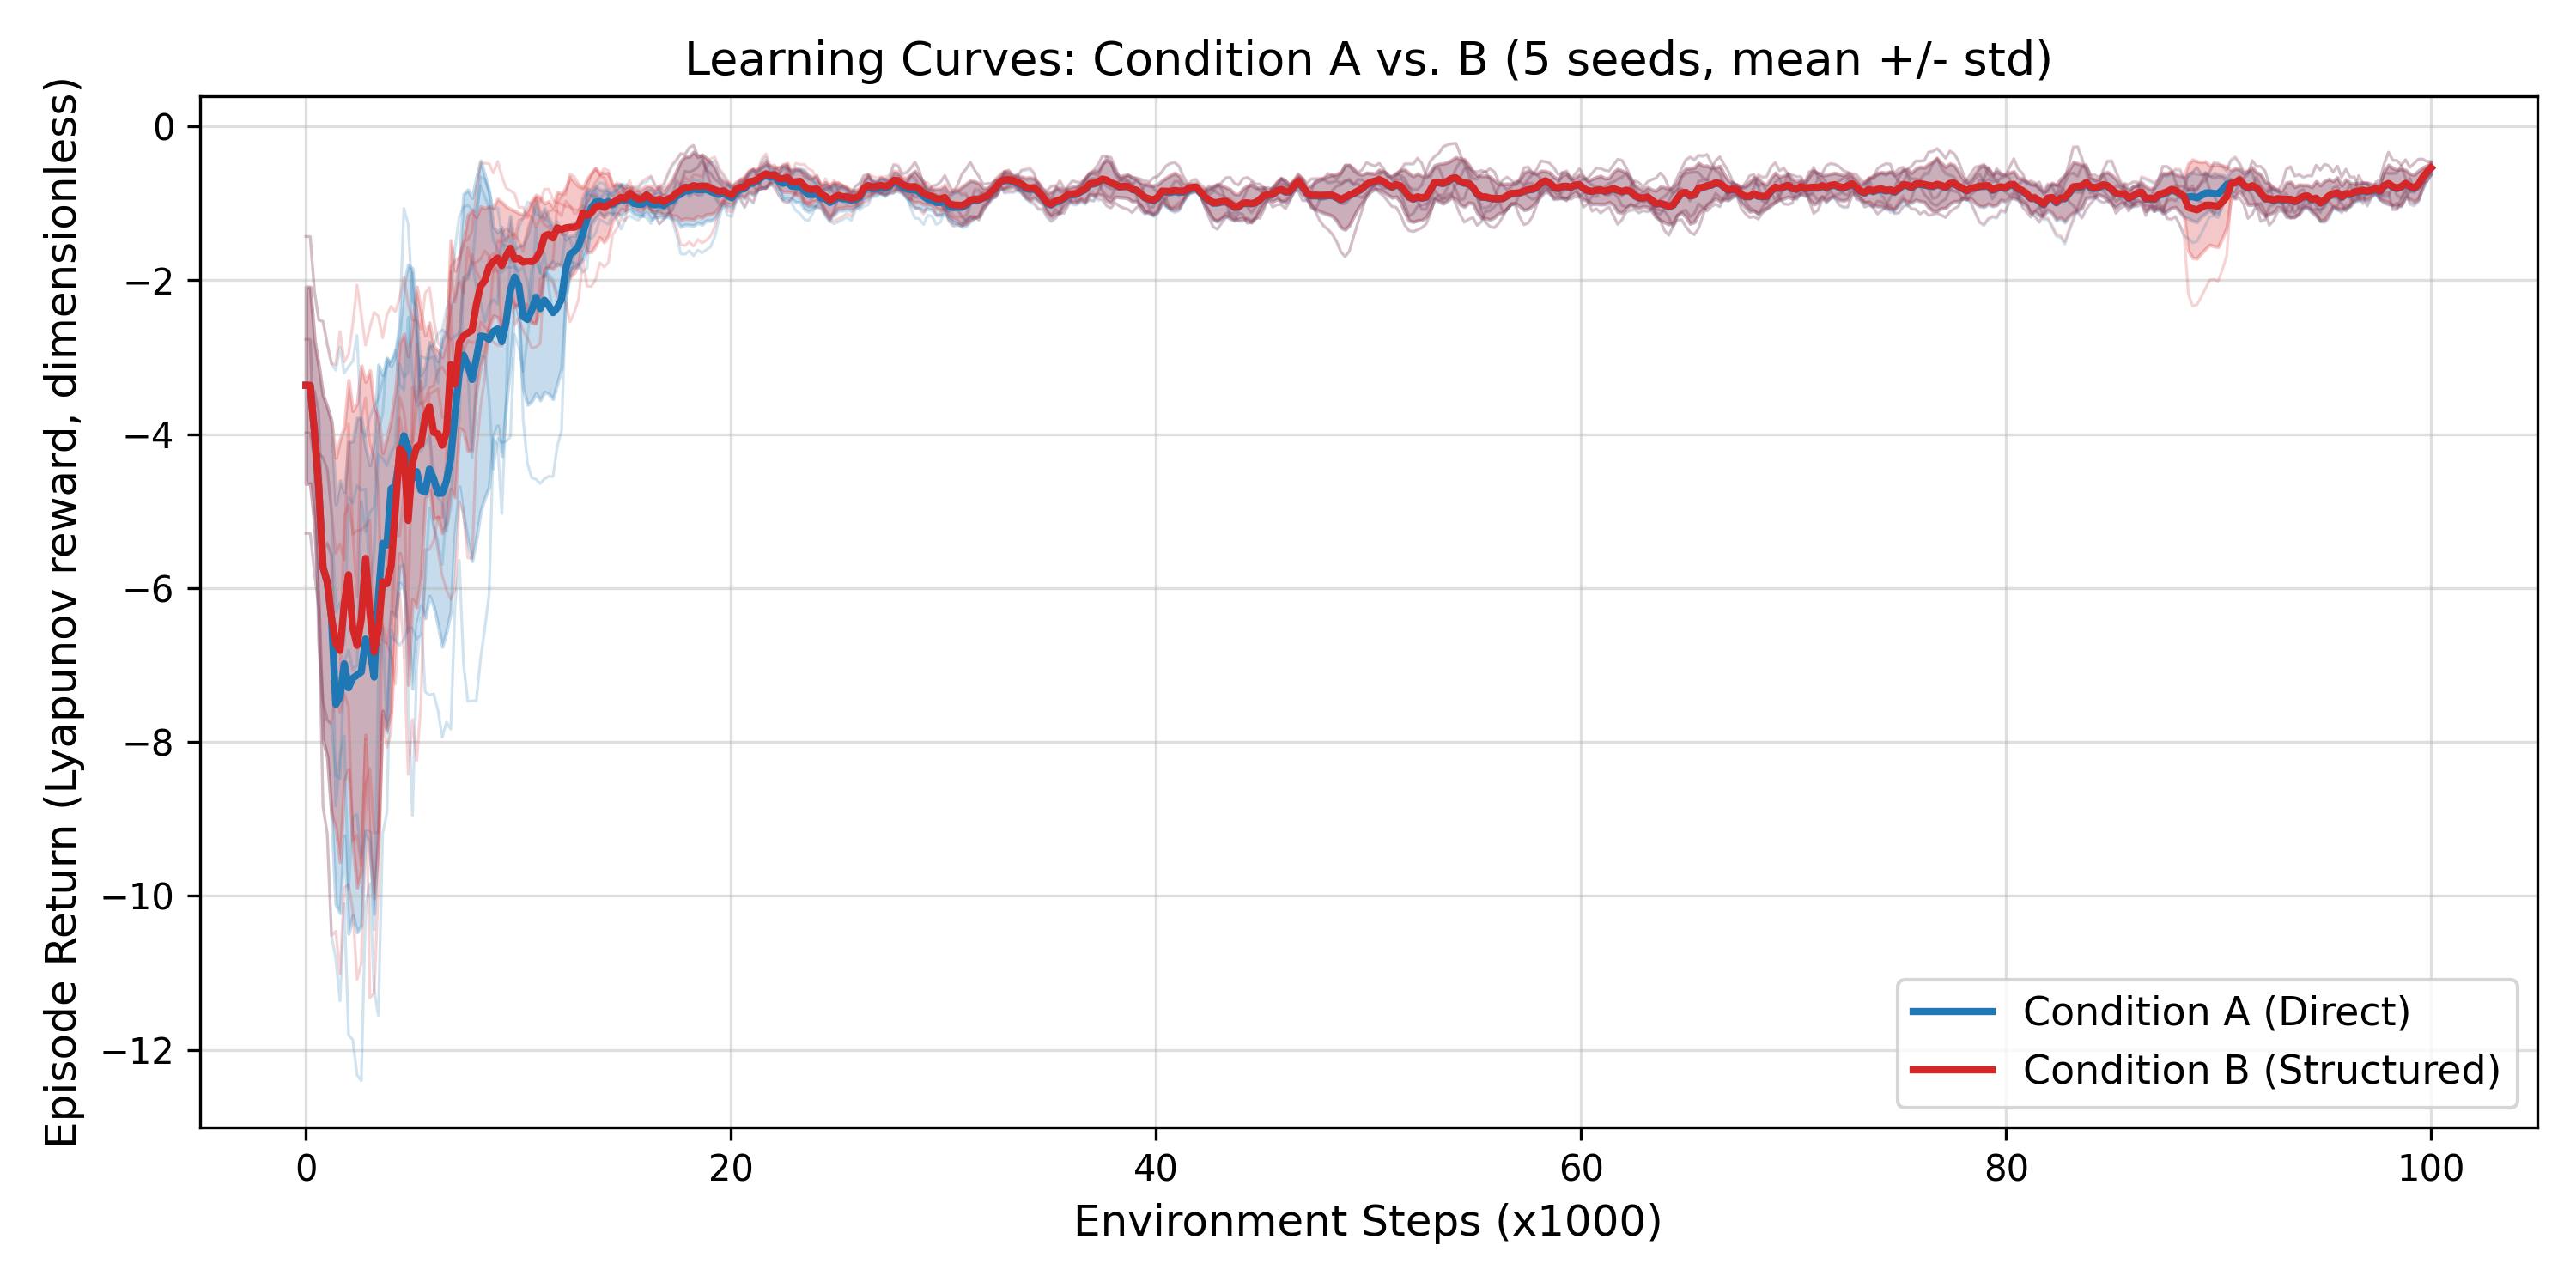
\includegraphics[width=0.75\linewidth]{Iteration2/input_files/plots/step_3_learning_curves_1_1776948522.png}
  \caption{Learning curves (mean $\pm$ std, 5 seeds) for Condition A (standard PPO critic) and Condition B (Lyapunov-structured critic $V(s)=\Phi(s)+f_\theta(s)$). Both conditions converge to similar episode returns within 100,000 steps.}
  \label{fig:learning_curves}
\end{figure}

\subsection{Critic Loss: MSE vs.~GAE Returns}
The most informative metric is the PPO critic training loss — the MSE between the predicted $V(s)$ and the GAE-computed returns $G_t$. Table~\ref{tab:critic_loss} reports this loss at different training phases.

\begin{table}[h]
  \centering
  \caption{Critic loss (MSE vs.~GAE returns) at different training phases. Condition B achieves 87\% lower overall loss and an 8$\times$ reduction in early training.}
  \label{tab:critic_loss}
  \begin{tabular}{lcc}
    \toprule
    Phase & Condition A & Condition B \\
    \midrule
    Early training (first 20\%) & 5.686 & \textbf{0.734} \\
    Final training (last 20\%)  & \textbf{0.0010 $\pm$ 0.0003} & 0.0029 $\pm$ 0.0051 \\
    Overall mean                & 1.057  & \textbf{0.136} \\
    \bottomrule
  \end{tabular}
\end{table}

Condition B achieves an 8-fold lower critic loss during early training (0.734 vs.~5.686), confirming that the Lyapunov prior provides a substantially better initialization for predicting actual discounted returns. Both conditions converge to similarly low final losses, but the early advantage is where sample efficiency is determined.

\subsection{Value Function Analysis}
Figure~\ref{fig:heatmaps} shows heatmaps of the analytic $\Phi(s)$, the learned $V_A(s)$, $V_B(s)$, and the residual $f_\theta(s)$ evaluated on a 100$\times$100 grid of states. The MSE between each learned value function and $\Phi(s)$ on this grid was: $\text{MSE}(V_A, \Phi) = 71.98$ vs.~$\text{MSE}(V_B, \Phi) = 10.07$ — an 86\% reduction. The learned residual $f_\theta(s)$ had a mean absolute magnitude of approximately 26\% of $\Phi(s)$, indicating non-trivial corrections beyond the Lyapunov prior.

\begin{figure}[h]
  \centering
  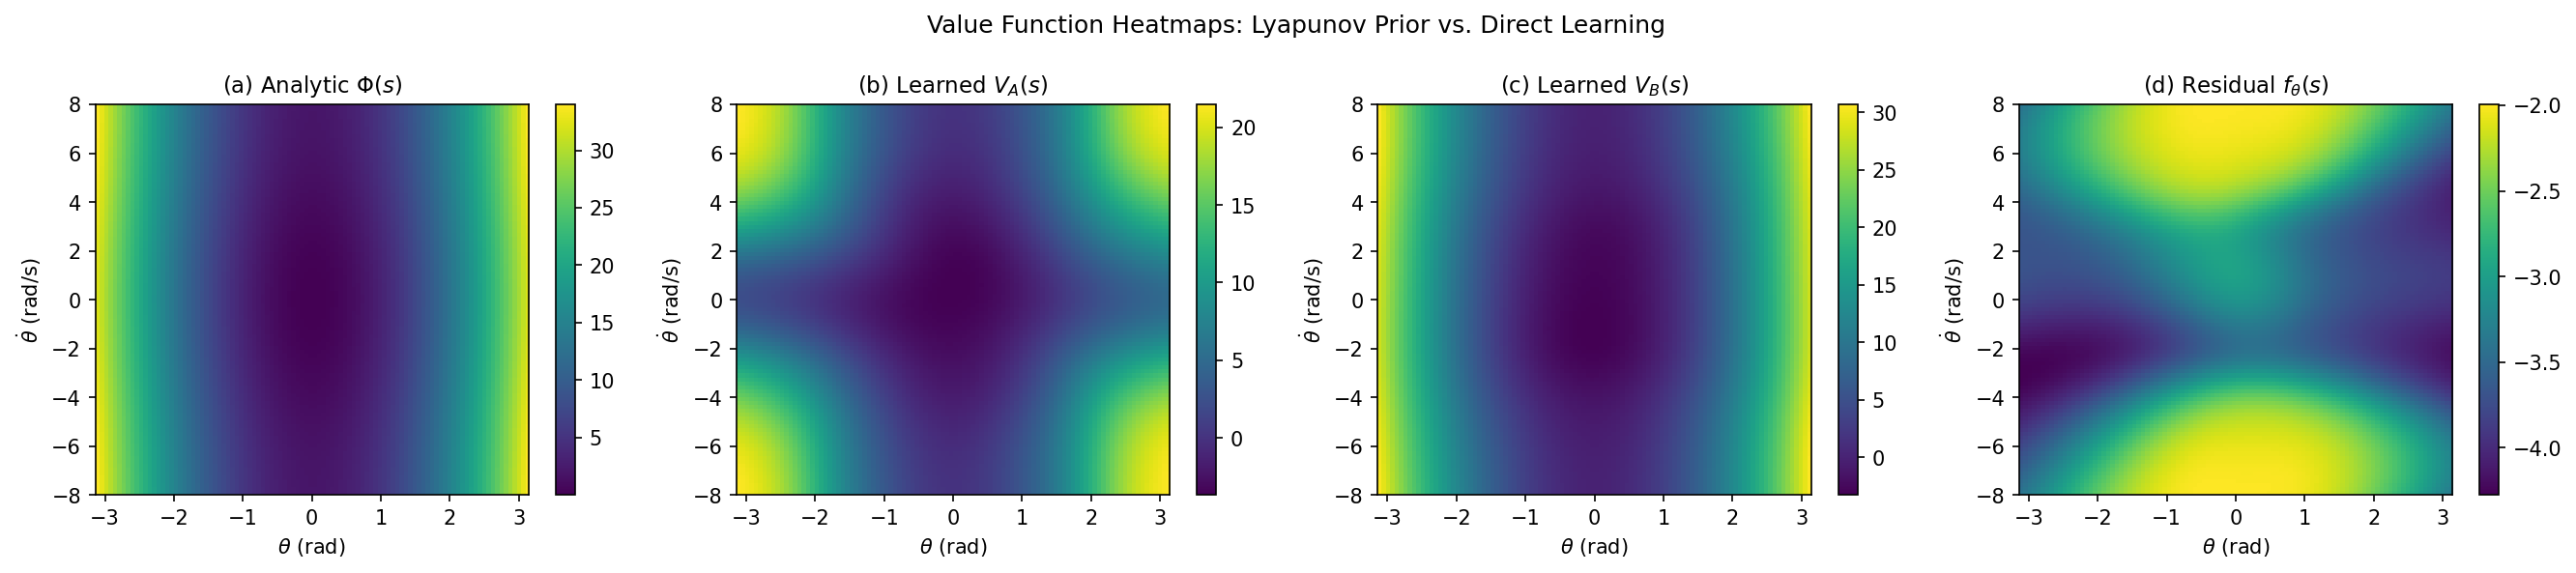
\includegraphics[width=\linewidth]{Iteration2/input_files/plots/value_function_heatmaps.png}
  \caption{Value function heatmaps over the $(\theta, \dot\theta)$ state space: (a) analytic $\Phi(s)$, (b) learned $V_A(s)$ (Condition A), (c) learned $V_B(s)$ (Condition B), (d) residual $f_\theta(s)$. Condition B is structurally much closer to $\Phi(s)$ ($\text{MSE} = 10.07$ vs.~$71.98$).}
  \label{fig:heatmaps}
\end{figure}

\subsection{Upright Stability and Summary}
Upright stability (fraction of evaluation steps with $|\theta| < 0.1$ rad) was near zero for both conditions: $0.0010 \pm 0.0018$ for Condition A and $0.0041 \pm 0.0038$ for Condition B. Neither policy reliably stabilizes the pendulum within the 100,000-step budget. Table~\ref{tab:summary} summarizes all metrics.

\begin{table}[h]
  \centering
  \caption{Summary of performance metrics across 5 seeds (mean $\pm$ std).}
  \label{tab:summary}
  \begin{tabular}{lcc}
    \toprule
    Metric & Condition A & Condition B \\
    \midrule
    Mean episode return      & $-0.778 \pm 0.168$ & $-0.775 \pm 0.167$ \\
    Overall critic loss (MSE vs.~returns) & 1.057 & \textbf{0.136} \\
    MSE($V$, $\Phi$) on state grid & 71.98 & \textbf{10.07} \\
    Mean upright fraction    & $0.0010 \pm 0.0018$ & $0.0041 \pm 0.0038$ \\
    \bottomrule
  \end{tabular}
\end{table}

\section{Conclusions}
\label{sec:conclusions}
This paper investigated the challenge of sample inefficiency in deep reinforcement learning for continuous control, focusing on the difficulty of learning accurate value functions from scratch. We proposed and evaluated a method to accelerate critic learning by incorporating control-theoretic domain knowledge. This was achieved by structuring the critic's value function as the sum of a known, analytical Lyapunov function and a learned neural network residual.

Our methodology involved applying the Proximal Policy Optimization (PPO) algorithm to the Gymnasium Pendulum-v1 stabilization task. To align the learning objective with the control goal, we defined the reward signal as the decrease in the system's energy, as described by the Lyapunov function. We then compared the performance of a standard PPO agent against an agent equipped with our proposed Lyapunov-structured critic over a 100,000-step training horizon.

The results demonstrated a clear and significant benefit of the structural prior on the critic's learning process. The Lyapunov-structured critic achieved an 87\% lower overall training loss and converged substantially faster, particularly in the early stages of training where its loss was 8 times lower than the baseline. Furthermore, the final learned value function was 86\% closer to the analytical Lyapunov function, confirming that the prior effectively guided the approximation. However, these dramatic improvements in value function approximation did not translate into superior policy performance or sample efficiency. The learning curves and final policy stability metrics were nearly identical for both agents, and neither learned to reliably stabilize the pendulum within the given training budget.

From these findings, we conclude that incorporating a Lyapunov function as a structural prior is a highly effective technique for accelerating the convergence of the value function in an actor-critic framework. It provides a strong, physically-meaningful initial estimate that the neural network only needs to refine. However, we also learned that for on-policy algorithms like PPO, rapid critic convergence does not guarantee a corresponding acceleration in policy improvement, at least not on shorter training horizons. The policy update mechanism may represent a separate bottleneck that requires more extensive environment interaction to leverage the more accurate value estimates provided by the structured critic. This suggests a potential decoupling between the learning speeds of the actor and the critic, a factor that warrants further investigation in the pursuit of more sample-efficient reinforcement learning.


\bibliography{bibliography}{}
\bibliographystyle{unsrt}

\end{document}
